% !TeX program = lualatex
% !TeX encoding = utf-8
% !TeX spellcheck = ru_RU
%==========================================================
% v.10
% Отчет может быть откомпилирован в LuaLaTeX.
% Например в дистирибутивах MikTeX или TeXlive
% (требуется установка пакета minted), а также
% в он-лайн версии https://www.overleaf.com/
% (включите компилятор LuaLaTeX).
%
% Для создания документа может потребоваться несколько
% запусков его компиляции. Например, обновление содержания
% требует двойной компиляции.
%
% Обратите внимание на команду команда сжатия/растяжения
% текста \textls из пакета microtype (см. пример).
%==========================================================
\documentclass[14pt]{extarticle}
\usepackage[main=russian,english]{babel}% языковая поддержка
\usepackage{unicode-math}% пакет для набора математики
\usepackage[explicit]{titlesec}% настройка заголовков
\usepackage{titletoc}% настройка содержания
\usepackage{enumitem}% настройка нумерованных списков
\usepackage{cite}% ссылки на литературу [1-10]
\usepackage[tracking=true]{microtype}% микротипографика
\microtypecontext{kerning=russian}% настройка микротипографики
\usepackage{geometry}% настройка геометрии страницы
\usepackage{graphicx}% поддержка графики
\usepackage{float}% для поддержки опции \begin{figure}[H]
%вставка не плавающего рисунка как в MS Word
\usepackage{indentfirst}% красная строка в первом абзаце
%========================================
\babelfont{rm}[Scale=0.976]{TimesNewRoman}% шрифт с засечками для кириллицы
% если нужен шрифт без засечек в документе, то подключаем его
%\babelfont{sf}[Scale=MatchLowercase]{Arial}% шрифт без засечек
% Scale=MatchLowercase - масштабировать выбранный шрифт в соответствии с
% текущим римским шрифтом по умолчанию до высоты строчных
\babelfont{tt}[Scale=0.976]{CourierNew}% моноширинный шрифт
%========================================
\usepackage{xcolor}% поддержка цвета
\usepackage{verbatim}% используем из этого пакета окружение comment для многострочных комментариев
\usepackage{tabularray}% для создания таблиц
\usepackage{tikz}% пакет для рисования
\usetikzlibrary{calc, decorations.pathmorphing, arrows, positioning, shapes, shapes.misc, fit}% библиотеки для пакета tikz
\usepackage[open, numbered]{bookmark}% закладки в pdf с нумерацией
\usepackage{fancyhdr}% настройка колонтитулов страницы
\usepackage{flafter}% помещает флоат ПОСЛЕ первой ссылки на него
\usepackage[section, above, below]{placeins}% вставить барьер для флоатов на границе с секцией
\usepackage{setspace}% определение интервала в тексте
\usepackage{needspace}% проверка места свобоного места и перенос на новую страницу
% Для предотвращения отрыва заголовка от многостраничного листинга
% \needspace{3\baselineskip} - три строки свободно
\usepackage[singlelinecheck=false]{caption}% настройка заголовков
\usepackage[newfloat]{minted}% листинги
\usepackage{xpatch}% для модернизации существующих команд
\usepackage{csquotes}% расширенная языковая поддержка
% нужно загружать последним
% https://tex.stackexchange.com/questions/326950/hyperref-conflicts-with-footnote
\usepackage{hyperref}% гипертекстовые ссылоки в документе
\usepackage[all]{hypcap}% подключать после hyperref
%========================================
\renewcommand{\UrlFont}{\ttfamily\small}% определене размера шрифта small для ссылок url
%========================================
\setlength{\parindent}{1.25cm}% Отступ красной строки
% Для отступов внутри заголовков глав, разделов и др. так как
% в них отступ может быть равен "0"
\newlength{\normalparindent} 
\setlength{\normalparindent}{\parindent}
%
\geometry{% настройка страницы, шрифтов и отступов
	a4paper,
	left=25mm,
	right=10mm,
	top=20mm,
	bottom=20mm,
	headsep=5mm,
%	showframe% показать поля страниц
}
%========================================
% отключение правил размещения плавающих
% объектов (рис., лист., табл.) по 10 на стринице
\setcounter{totalnumber}{10}
\setcounter{topnumber}{10}
% https://tex.stackexchange.com/questions/68516/avoid-that-figure-gets-its-own-page
% https://tex.stackexchange.com/questions/39017/how-to-influence-the-position-of-float-environments-like-figure-and-table-in-lat
\renewcommand{\topfraction}{.8}% (по умолчанию 0,7) максимальный размер верхней области для размещения поплавков
\renewcommand{\floatpagefraction}{.8}% (по умолчанию 0.5) минимальная часть страницы (или столбца), которая должна быть занята поплавками, чтобы иметь возможность сформировать поплавок (или столбец)
\renewcommand{\textfraction}{0}%(по умолчанию 0.2) минимальный размер текстовой области, т.е. площадь, которая не должна быть занята поплавками
%========================================
% подавление висячих строк в тексте
\clubpenalty=10000
\widowpenalty=10000
%========================================
\setstretch{
	0.976% одинарный интервал
%	1.464% полуторный интервал
}
%========================================
% настройка колонтитулов страницы
\pagestyle{fancy}
\fancyhf{}% очистка текущих значений
\setlength{\headheight}{0pt}
\fancyfoot[C]{\thepage}% номер страницы вверху по центру
\renewcommand{\headrule}{}% отключить линию в вверхнем колонтитуле
\fancypagestyle{plain}{% номер страницы в центре для 1-й страницы chapter
	\fancyfoot[C]{\thepage}
}
%========================================
% настройка оформления списков
\setlist{nosep, wide}% убрать вертикальные отступы, текст всю ширину
\setlist[enumerate]{label={\arabic*)}}% определяем оформление нумерованных списков
%========================================
% настройка заголовков у рисунков, таблиц и листингов
\DeclareCaptionLabelSeparator{defffis}{~--~}
%----------------------------------------
\captionsetup[table]{aboveskip=4pt plus 2pt minus 2pt, belowskip=4pt plus 2pt minus 2pt, margin={\normalparindent, 0pt}, indention=-\normalparindent, labelsep=defffis, font=normalsize}
%----------------------------------------
\captionsetup[figure]{aboveskip=4pt plus 2pt minus 2pt, belowskip=4pt plus 2pt minus 2pt, justification=centering, labelsep=defffis, font=normalsize}
%----------------------------------------
\captionsetup[listing]{aboveskip=4pt plus 2pt minus 2pt, belowskip=4pt plus 2pt minus 2pt, margin={\normalparindent, 0pt}, indention=-\normalparindent, labelsep=defffis, font=normalsize}
%----------------------------------------
% настройка заголовков для многостраничных таблиц longtblr пакет tabularray
\DefTblrTemplate{firsthead}{default}{\addtocounter{table}{-1}\captionof{table}[\InsertTblrText{entry}]{\InsertTblrText{caption}}}
\DefTblrTemplate{middlehead,lasthead}{default}{\addtocounter{table}{-1}\captionof{table}[]{\InsertTblrText{caption}~(Продолжение)}}
\DefTblrTemplate{contfoot-text}{default}{\centerline{Продолжение на следующей странице}}
\SetTblrTemplate{caption-lot}{empty}
%========================================
% настройка визуализации листингов
% https://pygments.org/demo/#try - тут можно попробовать разные стили
\setminted{xleftmargin=0.5cm, linenos, numbersep=5pt, breaklines, breakanywhere, frame=single, framesep=1ex, fontsize=\small}% настройки оформления листингов
%----------------------------------------
% создание окружения code для оформления
% многостраничных листингов
\newenvironment{code}{\captionsetup{type=listing}}{}
\SetupFloatingEnvironment{listing}{name=сode}
% проверяем свободное место в 3 baselineskip, если меньще,
% то выпоняется перенос на следующую страницу, а также
% определяем одинарный итервал \setstretch{1}\selectfont
\AtBeginEnvironment{code}{\needspace{3\baselineskip}\setstretch{1}\selectfont}
%----------------------------------------
% добавляем команду отключающую лишние вертикальные отступы в листингах \fvset{vspace=0pt}
% и команду определяющую одинарный интервал \setstretch{1}\selectfont
% перед командой inputminted
\xpretocmd{\inputminted}{\fvset{vspace=0pt}\setstretch{1}\selectfont}{}{}% при загрузке из внешнего файла
\BeforeBeginEnvironment{minted}{\fvset{vspace=0pt}\setstretch{1}\selectfont}% при использовании окружения \begin{minted} \end{minted}
%========================================
% команда удалемния пробела после окружения
\newcommand{\nospacebetweenenvs}{\vspace{-\glueexpr(\topsep+\partopsep)*2}}
%========================================
% определяем стандартные названия
\addto\captionsrussian{\def\figurename{Рис.}}% подпись для рисунка
\addto\captionsrussian{\def\tablename{Табл.}}% подпись для таблицы
\addto\captionsrussian{\def\listingname{Лист.}}% подпись для листинга
%========================================
\makeatletter
%========================================
\newcommand{\hrf}[1]{\hbox to #1{\hrulefill}}% команда подчеркивания
%========================================
% настройка заголовков и их отоборажения в содержании
\renewcommand{\@pnumwidth}{1.25em}% настройка отступа под номер страницы в содержании
% настройка оформления в тексте и содержании для section
\titleformat{\section}[block]
{\hspace*{\normalparindent}\normalfont\bfseries}
{\thesection}
{1ex}
{#1}
[]
%
\titlespacing*{\section}{0pt}{14pt plus 3pt minus 3pt}{14pt plus 3pt minus 3pt}
%
\titlecontents{section}
[0pt]
{}
%{\makebox[1.25em][l]{\thecontentslabel}}% второй вариант оформления
{\contentspush{\makebox[1.25em][l]{\thecontentslabel}}}% второй вариант оформления: добавляет отступ под номер для всех строк заголовка в содержании (смотреть на многострочных заголовках)
{}
{\nolinebreak\titlerule*[1pc]{.}\contentspage}% \nolinebreak добавлен для предотвращения нежелательных разрывов строк между заголовками и номерами страниц
[]
%========================================
% создание нового вида секции в документе
\newcounter{sectionc}% создание счетчика для sectionc
\titleclass{\sectionc}{straight}[\part]% создание новой секции sectionc
% секция sectionc является подчиненной \part
% для класса article ToC level(part)=0, тогда ToC level(sectionc)=1
% т.е. ToC level(section)=ToC level(sectionc)
% straight - означает, что секция может быть использовна
% в любом месте страницы
% настройка оформления в тексте и содержании для sectionс
\titleformat{\sectionc}[block]
{\normalfont\bfseries}
{}
{0pt}
{\filcenter #1}
[]
%
\titlespacing*{\sectionc}{0pt}{14pt plus 3pt minus 3pt}{14pt plus 3pt minus 3pt}
%
\titlecontents{sectionc}
[0em]
{\normalfont}
{}
{}
{\nolinebreak\titlerule*[1pc]{.}\contentspage}
[]
%========================================
% для корректного вывода закладок в PDF при просмотре
\def\toclevel@sectionc{1}% настройка уровня нового вида секций
% команды для вкл/откл номера в закладках
\newcommand{\numbersections}{\renewcommand{\Hy@numberline}[1]{##1~}}
\newcommand{\nonumbersections}{\renewcommand{\Hy@numberline}[1]{}}
% включаем нумерацию для section переопределяя команду
\let\oldsection\section
\renewcommand{\section}{\numbersections\oldsection}
% отключаем нумерацию для sectionc переопределяя команду
\let\oldsectionc\sectionc
\renewcommand{\sectionc}{\nonumbersections\oldsectionc}
%========================================
% содержание по центру
\renewcommand\tableofcontents{
	\pdfbookmark[sectionc]{\contentsname}{toc} % Добавляем Содержание в закладку PDF ToC
	\sectionc*{\contentsname
		\@mkboth{\contentsname}{\contentsname}}
	\@starttoc{toc}
}
%========================================
% настройка списка литературы
\renewenvironment{thebibliography}[1]{
	\sectionc{Список использованных источников}
	\@mkboth{\MakeUppercase\refname}{\MakeUppercase\refname}%
	\begin{enumerate}[label=\arabic*., fullwidth, nosep, itemindent=\parindent, 
		listparindent=\parindent]
		\@openbib@code
		\sloppy
		\clubpenalty4000
		\@clubpenalty \clubpenalty
		\widowpenalty4000
		\sfcode`\.\@m}
	{\def\@noitemerr
		{\@latex@warning{Empty `thebibliography' environment}}%
\end{enumerate}}
%========================================
% элементы блок-схемы
\tikzstyle{adds} = [minimum height=2em, minimum width=12em]
\tikzstyle{terminator} = [rectangle, draw, align=center, rounded corners, fill=blue!25, adds]
\tikzstyle{process} = [rectangle, draw, align=center, fill=red!25, adds]
\tikzstyle{data}=[trapezium, draw, align=center, trapezium left angle=70, trapezium right angle=-70, trapezium stretches body, fill=green!25, adds]
\tikzstyle{decision} = [diamond, draw, aspect=1.5, align=center, text badly centered, fill = yellow!25]
\tikzstyle{connector} = [draw, -stealth]
\tikzstyle{ciclestart} = [chamfered rectangle,chamfered rectangle corners={north west, north east}, chamfered rectangle xsep=0.8em, draw, align=center, fill=orange!25, adds]
\tikzstyle{cicleend} = [chamfered rectangle,chamfered rectangle corners={south west, south east}, chamfered rectangle xsep=0.8em, draw, align=center, fill=orange!25, adds]
\tikzstyle{adds} = [minimum height=2em, minimum width=12em]
%========================================
% настройка отступов вокруг уравнений
% в данной настройке уменьшено в 2 раза
% относительно стандартных
\AtBeginDocument{%
	\abovedisplayskip=6pt plus 1.5pt minus 4.5pt
	\abovedisplayshortskip=0pt plus 1.5pt
	\belowdisplayskip=6pt plus 1.5pt minus 4.5pt
	\belowdisplayshortskip=3.5pt plus 1.5pt minus 2pt 
}
%========================================
% Настройка вертикальных отступов до, после и между плавающими рисунками
\AtBeginDocument{%
% вертикальное расстояние между двумя флоатс (около 12pt)
\setlength{\floatsep}{7pt plus 3pt minus 3pt}
% расстояние между флоатс (в верхней или нижней части страницы) и текстом (по умолчанию, около 20pt)
\setlength{\textfloatsep}{7pt plus 3pt minus 3pt}
% расстояние между флоатс вставленным "прямо здесь" (параметр h) и текстом (около 12pt)
\setlength{\intextsep}{7pt plus 3pt minus 3pt}
%  расстояние над и под подписью к флоат
%\setlength{\abovecaptionskip}{0pt}
%\setlength{\belowcaptionskip}{0pt}
%\setlength{\floatsep}{0pt}
%\setlength{\textfloatsep}{0pt}
%\setlength{\intextsep}{0pt}
}
%========================================
\makeatother
\graphicspath{{pic/}}% папка с рисунками
\begin{document}
%%%%%%%%%%%%%%%%%%%%%%%%%%%%%%%%%%%%
%                                  %
%          Титульный лист          %
%                                  %
%%%%%%%%%%%%%%%%%%%%%%%%%%%%%%%%%%%%
% Выравнивание контента по центру можно делать разными способами
% \centerline{...} - выравнивает строку по центру (для одной строки!)
% \begin{center} - окружение для выравнивания по центру (добавлят вертикальный отступы до и после)
%  ...
% \end{center}
% {\par\centering - окружение для выравнивания по центру без добавления вертикальных отступов
% ...
% \par}
{\par\centering% окружение для выравнивания по центру


\includegraphics[width=0.12\linewidth]{logo.pdf}% вставляем логотип

МИНИСТЕРСТВО ЦИФРОВОГО РАЗВИТИЯ, СВЯЗИ И\\МАССОВЫХ КОММУНИКАЦИЙ РОССИЙСКОЙ ФЕДЕРАЦИИ\\[5mm]% новый абзац + отступ 5мм
% \textbf - делает шрифт жирным

Ордена Трудового Красного Знамени федеральное государственное\\ бюджетное образовательное учреждение высшего образования\\ «\textbf{Московский технический университет связи и информатики}»\\(\textbf{МТУСИ})\\[5mm] 
	
Кафедра «Системное программирование»
\par}

\begin{tikzpicture}[overlay, remember picture] % рисуем рамку на титульнике
	\draw[line width=0.5mm] 
	($(current page.north west) + (20mm, -10mm)$)
	rectangle
	($(current page.south east) + (-10mm, 10mm)$);
%	\node [inner sep=0pt] (img) at ($(current page.south east) + (-76mm, 61.5mm)$)	{\includegraphics[width=2cm]{pic/polsign.png}};% добавляем подпись преподавателя
\end{tikzpicture}


\vfill\vfill% двойной бесконечный вертикальный промежуток (работает как пружина)

{\par\centering
\textbf{ОТЧЕТ}\\ по лабораторной работе №\,7\\[5mm]

дисциплина «\textbf{Математические основы баз данных}»\\[5mm]
\textcolor{red}{\textit{Версия документа v.\,10}}
\par}

\vfill% бесконечный вертикальный промежуток

\hfill% бесконечный горизонтальный промежуток (работает как пружина)
\begin{minipage}{0.45\textwidth}% министраница шириной 0.45 от ширины текста
	Выполнил:\\[2mm]
	студент гр.\,БФИхххх\\[2mm]
	\hrf{2.7cm}\,Фамилия И.\,О.\\[2mm]
	«\,\hrf{1cm}\,»\,\hrf{2.5cm}\,\the\year{}\,г.\\
	
	Проверил:\\[2mm]
	д.т.н., профессор\\[2mm]
	\hrf{2.7cm}\,Полищук Ю.\,В.\\[2mm]
	«\,\hrf{1cm}\,»\,\hrf{2.5cm}\,\the\year{}\,г.
\end{minipage}

\vfill

\centerline{Москва, \the\year{}\,г.}% строка по центру
\thispagestyle{empty}% стиль страницы отсутствует (без номера страницы)
%%%%%%%%%%%%%%%%%%%%%%%%%%%%%%%%%%%%
%                                  %
%            Содержание            %
%                                  %
%%%%%%%%%%%%%%%%%%%%%%%%%%%%%%%%%%%%
\newpage% новая страницы
\tableofcontents% содержание
%%%%%%%%%%%%%%%%%%%%%%%%%%%%%%%%%%%%
%                                  %
%         Тело документа           %
%                                  %
%%%%%%%%%%%%%%%%%%%%%%%%%%%%%%%%%%%%
\newpage% новая страница
\sectionc{Введение}% секция по центру без номера

Современное информационное поле состоит из массы событий, объектов и явлений. Оно охватывает такие объемы, что без четко действующей определенной системы, хранение всех этих данных могло быть хаотичным и неуправляемым\cite{kon2017}. % ссылка на статью из библиографии

База данных (\textbf{БД}) реализует собой способ обработки информации, и используется во всех сферах человеческой жизни.

Таким образом, повышение эффективности функционирования \textbf{БД} является актуальной задачей.

\section{Цель работы}% создание секции с номером
%\section[Очень очень очень очень очень очень очень очень очень\protect\\ длинная цель работы]{Очень очень очень очень очень очень очень очень\\ очень длинная цель работы} % если нужно добавить разрыв строки (абзац) в названии секции в содержании, то это можно сделать с помощь команды \protect в необязательном параметре [], который передается в содержание

Изучения возможностей улучшения производительности \textbf{БД}.

\section{Задание}

\textls[-5]{Для \textbf{БД} создать необходимые индексы и продемонстрировать увеличение скорости выполнения запросов. Отчет должен содержать титульный лист, задание, команды создания индексов, примеры запросов и результаты их выполнения, список использованных источников, нумерацию страниц, содержание, введение и заключение.}% использована команда сжатия/растяжения текста \textls (cжатие с "-", растяжение с "+")

\section{Реализация}

В процессе выполнения лабораторной работы использованы следующие информационные источники\cite{docpsql, nikov2020, rogov2020, morguniv2018}.

\sectionc*{Теоретические основы} % * показывает, что секция не попадает в содержание

В \textbf{PostgreSQL} при создании индекса по умолчанию он реализуется посредством \textbf{Б-дерева} (BTtree).


\textbf{Б-дерево} представляет собой сильно ветвящееся дерево, обладающее следующими свойствами:
\begin{enumerate}[label=--]% список без немерации
	\item каждая вершина может содержать не более $2n$ ключей;
	\item каждая вершина, за исключением, может быть, корневой, содержит не менее $n$ ключей (корневая вершина, если она не является листом, содержит не менее двух потомков);
	\item каждая вершина либо представляет собой лист и не имеет потомков, либо имеет в точности $m + 1$ потомка, где $m$~-- количество ключей в вершине;
	\item все листовые вершины располагаются на одном уровне. 
\end{enumerate}

Каждая не листовая вершина \textbf{Б-дерева} имеет вид (\ref{eq:btree}).% ссылка на метку
\begin{equation}% выражение с нумерацией и меткой
<p_0, k_1, p_1, k_1, \ldots, p_{m-1}, k_m, p_m>,
\label{eq:btree}
\end{equation}
где $p_i$ представляет собой указатель на $i$-го потомка, а $k_i$~-- значение ключа поиска (указатели на записи не указаны).

Для любого $i\in[1,m-1]$ все ключи, расположенные в поддереве, на которое указывает указатель $p_i$, находятся в диапазоне $[k_i, k_{i+1}]$. Ключи поддерева $p_0$ будут меньше $k_1$, а все ключи поддерева $p_m$~-- больше $k_m$.

Рассмотрим пример \textbf{Б-дерева} второго порядка $n = 2$ (рис.~\ref{f:btree}).

% Для размещения рисунка в документе используем окружение \begin{figure} \end{figure}.
% Внутри окружения делаем выравнивание по центру \centering.
% Вставляемый объект плавающий с опциями "!htpb".
% Если нужен не плавающий как в MS Word, то нужно использовать опцию H.
% Подробнее про плавающие объекты написанов тут:
% https://tex.stackexchange.com/questions/39017/how-to-influence-the-position-of-float-environments-like-figure-and-table-in-lat (англ.)
% https://mydebianblog.blogspot.com/2013/03/amorua-advanced-floats.html (рус.)
\begin{figure}[!htpb]
  \centering
  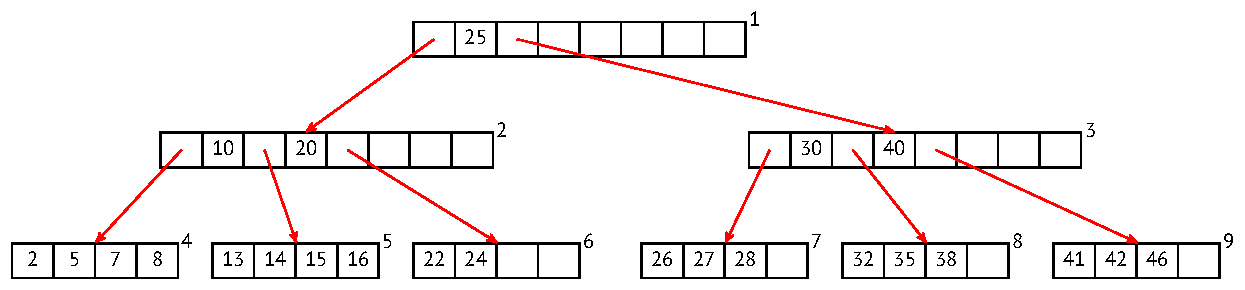
\includegraphics[width=1.0\linewidth]{MTUCIfig.pdf}
  \caption{Структура информационного наполнения документа\label{f:btree}}
\end{figure}

Для рассмотренной схемы (рис.~\ref{f:btree}): $1\ldots3$~-- корневые вершины, $4\ldots9$~-- листовые вершины.

Поиск ключа в \textbf{Б-дереве} происходит следующим образом. Начиная с корневой вершины, выполняются действия:
\begin{enumerate} % нумерованный список
	\item просматриваются ключи $k_1, k_2, \ldots, k_m$, если искомый ключ найден, то по указателю извлекается запись основного файла;
	\item \textls[-10]{если $k_i<k<k_{i+1}$ для $i\in[1,m]$, то поиск продолжается на странице $p_i$;}% использована команда сжатия/растяжения текста \textls (cжатие с "-", растяжение с "+")
	\item если $k<k_1$, то поиск продолжается на странице $p_0$;
	\item если $k>k_m$, то поиск продолжается на странице $p_m$.   
\end{enumerate}

\sectionc*{Практическая реализация} % * показывает, что секция не попадает в содержание

Продемонстрируем работу индекса для таблицы \mintinline{postgresql}{sgroup}. Добавим в нее таблицу 1\,млн. записей, сгенерированных случайным образом. Для этого воспользуемся скриптом, который представлен далее (лист.~\ref{lst:crandinsdemo}).

% Для размещения листинга в документе используем окружение \begin{listing} \end{listing}.
% Это позволит сделать его оформление аналогичным с рисунками и таблицами.
\begin{listing}[!htpb]
  \caption{Создаем и заполняем демонстрационную таблицу \mintinline{postgresql}{sgroup}\label{lst:crandinsdemo}}  
   % определяем язык листинга и вставляем листинг из внешнего файла из папки list
  \inputminted{postgresql}{list/demoindexadd.txt}  
\end{listing}


Сделаем выборку данных из таблицы для группы \mintinline{postgresql}{'02ИН'} с выводом статистики (лист.~\ref{lst:demoindexselect1}).

% Для размещения листинга в документе используем окружение \begin{listing} \end{listing}.
% Это позволит сделать его оформление аналогичным с рисунками и таблицами.
\begin{listing}[!htpb]
  \caption{Выборка данных из таблицы \mintinline{postgresql}{sgroup} (без индекса)\label{lst:demoindexselect1}}
  % определяем язык листинга и вставляем листинг из внешнего файла из папки list
  \inputminted{postgresql}{list/demoindexselect1.txt}
\end{listing}

Статистика запроса без использования индекса (лист.~\ref{lst:noindexqueryplan}).

% Для размещения листинга в документе используем окружение \begin{listing} \end{listing}.
% Это позволит сделать его оформление аналогичным с рисунками и таблицами.
\begin{listing}[!htpb]
  \caption{Статистика запроса (без индекса)\label{lst:noindexqueryplan}}
  % определяем язык листинга и вставляем листинг из внешнего файла из папки list
  \inputminted{postgresql}{list/noindexqueryplan.txt}
\end{listing}

Создаем индекс для поля таблицы, обновляем статистику по таблице и повторно выполняем выборку данных из таблицы с выводом статистики (лист.~\ref{lst:demoindexcreate}).

% Для размещения листинга в документе используем окружение \begin{listing} \end{listing}.
% Это позволит сделать его оформление аналогичным с рисунками и таблицами.
\begin{listing}[!htpb]
  \caption{Создание индекса, обновление статистики по таблице, выборка данных из таблицы (с использованием индекса)\label{lst:demoindexcreate}}
  % определяем язык листинга и вставляем листинг из внешнего файла из папки list
  \inputminted{postgresql}{list/demoindexcreate.txt}
\end{listing}

% барьер для плавающих флоатов
% может понадобится, чтобы разрядить очередь из флоатов
% данным пример можно посмотреть для 1.5 интервала текста
% включив и отключив команду FloatBarrier
%\FloatBarrier

Статистика запроса с использования индекса (лист.~\ref{lst:yesindexqueryplan}).

% Для размещения листинга в документе используем окружение \begin{listing} \end{listing}.
% Это позволит сделать его оформление аналогичным с рисунками и таблицами.
\begin{listing}[!htpb]
  \caption{Статистика запроса (с использованием индекса)\label{lst:yesindexqueryplan}}
  % определяем язык листинга и вставляем листинг из внешнего файла из папки list
  \inputminted{postgresql}{list/yesindexqueryplan.txt}
\end{listing}


В результате выполнения выборки данных из таблицы \textbf{БД} без использования индекса и с его применением были получены следующие результаты (табл.~\ref{t:tab1}).

% Для размещения листинга в документе используем окружение \begin{table} \end{table}.
% Это позволит сделать его оформление аналогичным с рисунками и листингами.
\begin{table}[!htpb]
	\centering
	\caption{Сравнение результатов выборки данных из таблицы\label{t:tab1}}
	\begin{tabular}{|p{0.33\textwidth}|c|c|}
	\hline
	~&\textbf{Без индекса}&\textbf{C индексом}\\
	\hline
	Время планирования (мс)&0.056&0.165\\
	\hline
	Время исполнения (мс)&80.452&0.066\\
	\hline
	\end{tabular}
\end{table}

Анализ данной таблицы показывает существенное увеличение скорости исполнения выборки при использовании индекса.

\sectionc{Заключение}

В процессе выполнения лабораторной работы была продемонстрирована эффективность применения индексов для реализации информационных запросов к \textbf{БД}, которая заключается в существенном повышении скорости их выполнения.

%%%%%%%%%%%%%%%%%%%%%%%%%%%%%%%%%%%%
%                                  %
%      Список источников           %
%                                  %
%%%%%%%%%%%%%%%%%%%%%%%%%%%%%%%%%%%%
\begin{thebibliography}{10} % Количество источников не более 10
\bibitem{kon2017}
Конюхов В.\,Г. База данных. Понятие, значение и роль в современном мире~// Системные технологии.~-- 2017.~-- №\,24.~-- С.\,61-63.

\bibitem{docpsql}
Официальная документация PostgreSQL URL:~\url{https://postgrespro.ru/docs?ysclid=ldeiuoyqev648714874} (дата обращения: 31.01.2023). % вставка ссылки на сайт

\bibitem{nikov2020}
Новиков Б.\,А. Основы технологий баз данных: учеб. пособие / Б.\,А. Новиков, Е.\,А. Горшкова, Н.\,Г. Графеева; под ред. Е.\,В. Рогова.~-- 2-е изд.~-- М.: ДМК Пресс, 2020.~-- 582\,с.

\bibitem{rogov2020}
Рогов Е.\,В. PostgreSQL изнутри.~-- М.: ДМК Пресс, 2022.~-- 660\,с.

\bibitem{morguniv2018}
Моргунов Е.\,П. PostgreSQL. Основы языка SQL: учеб. пособие / Е.\,П. Моргунов; под ред. Е.\,В. Рогова, П.\,В. Лузанова.~-- СПб.: БХВ-Петербург, 2018.~-- 336\,с.
\end{thebibliography}

%\begin{comment}% начало многострочного комментария
\newpage% новая страницв
\sectionc*{Дополнительные примеры оформления контента}

В данном разделе рассмотрены дополнительные примеры, которые могут быть использованы для оформления контента в отчете.

Рассматриваемую часть документа можно в удалить в итоговом \textbf{PDF}-документе использовав для этого окружение многострочного комментария \mintinline{tex}{\begin{comment}} \ldots \mintinline{tex}{\end{comment}}.

\noindent\textcolor{red}{\rule{\textwidth}{2pt}}% красная линия \noindent - убрать абзацный отступ

% установка для шрифта \bfseries - жирный, \itshape - курсив, \ttfamily - моноширинный шрфит
Пример \textcolor{red}{\bfseries использования русских индексов в формуле}:% цветной текст + жырный шрифт

\begin{equation}
	F^H (D^m) = -\log_2\left(
	\frac{F_\textup{ст}(P^\alpha_\textup{ст}) + F_\textup{дин}(P^\alpha_\textup{дин})}
	{2 \cdot \left(F_\textup{ст}(GP^\alpha_\textup{ст}(T_\textup{э})) + F_\textup{дин}(GP^\alpha_\textup{дин}(T_\textup{э})
		)\right)} + 0.5 \right),
	\label{eq:fentrop}
\end{equation}
где $F_\textup{ст}(P^\alpha_\textup{ст})$~-- функция, вычисляющая сумму весовых коэффициентов для статических параметров; $F_\textup{дин}(P^\alpha_\textup{дин})$~-- функция, вычисляющая сумму весовых коэффициентов для динамических параметров с учетом их <<устаревания>>; $GP^\alpha_\textup{ст}(T_\textup{э})$~-- функция, генерирующая множество теоретически возможных статических параметров системы за время эксплуатации $T_\textup{э}$; $GP^\alpha_\textup{дин}(T_\textup{э})$~-- функция, генерирующая множество теоретически возможных динамических параметров за время эксплуатации $T_\textup{э}$.

\noindent\textcolor{red}{\rule{\textwidth}{2pt}}

Интеграция листинга в документ \textcolor{red}{\bfseries без использования внешнего файла} (лист.~\ref{lst:nofile}).

% Для размещения листинга в документе используем окружение \begin{minipage} \end{minipage}.
% Это позволит сделать его оформление аналогичным с рисунками и таблицами.
% Для непосредственной вставки листинга используем окружение \begin{minted} \end{minted}
\begin{listing}[!htpb]
\caption{Интеграция листинга без использования внешнего файла\label{lst:nofile}}
\begin{minted}{postgresql}
select s.last_name
from student s, student_hobby sh, hobby h
where s.id=sh.id_student and sh.id_hobby=h.id
group by 1
having count(sh.id_hobby)>1;
\end{minted}
\end{listing}

\noindent\textcolor{red}{\rule{\textwidth}{2pt}}

Пример интеграции \textcolor{red}{\bfseries многостраничного листинга} (лист.~\ref{lst:dbstart}).

% для проверки автопереноса названия
% перенос после отступа в 13 baselineskip
%\vspace{12\baselineskip}
%
% Для размещения многостраничного листинга используем окружение \begin{code} \end{code}.
\begin{code}
	\caption{Скрипт демонстрационной \textbf{БД}\label{lst:dbstart}}
	\inputminted{postgresql}{list/dbstart.txt}
\end{code}

\noindent\textcolor{red}{\rule{\textwidth}{2pt}}

Результаты выполнения запроса можно визуализировать в отчете следующим образом (лист~\ref{lst:visual}).

% Для размещения листинга в документе используем окружение \begin{listing} \end{listing}.
% Это позволит сделать его оформление аналогичным с рисунками и таблицами.
\begin{listing}[!htpb]
  \caption{Пример результата запроса\label{lst:visual}}
  % определяем язык листинга и вставляем листинг из внешнего файла из папки list
  \inputminted[xleftmargin=0cm, linenos=false, numbersep=0pt, fontsize=\small]{text}{list/demoresult.txt}
\end{listing}

\noindent\textcolor{red}{\rule{\textwidth}{2pt}}

Существует множество пакетов для создания таблиц. Создадим таблицу во всю ширину страницы и продемонстрируем выравнивания текста внутри ячеек с помощью пакета \mintinline{latex}{tabular} (табл.~\ref{t:tab2}).

% Для размещения листинга в документе используем окружение \begin{table} \end{table}.
% Это позволит сделать его оформление аналогичным с рисунками и листингами.
\newlength\q% создаем переменную длины
% определяем ее размер для ячейки с учетом столбцов-разделителей 2\tabcolsep
\setlength\q{\dimexpr 0.33\textwidth - 2\tabcolsep}
\begin{table}[!htpb]
	\centering
	\caption{Пример таблицы во всю ширину с выравниванием\label{t:tab2}}
	\begin{tabular}{|p{\q}|p{\q}|p{\q}|} % три колонки
		\hline
		По левому краю \hfill & \hfil В центре & \hfill По правому краю \\
		\hline
		Существует\par множество пакетов\par для рисования таблиц & ~\par\hfil 1.00 & \hfil 2.00 \\
		\hline
		Существует множество пакетов для рисования таблиц & ~\par\hfil 3.00 & ~\par~\par\hfil 4.00 \\
		\hline
	\end{tabular}
\end{table}

\noindent\textcolor{red}{\rule{\textwidth}{2pt}}

Используя пакет \mintinline{latex}{tabularray} создаем таблицу во всю ширину страницы в которой текст второй строки выделен жирным шрифтом и определена пропорция для размера ячеек (табл.~\ref{t:tab4}).

% Для размещения листинга в документе используем окружение \begin{table} \end{table}.
% Это позволит сделать его оформление аналогичным с рисунками и листингами.
\begin{table}[!htpb]
	\centering
	\caption{Пример таблицы с использованием \mintinline{latex}{tabularray}\label{t:tab4}}
	\begin{tblr}{
			width = 1.0\textwidth, colspec = {X[1]X[1]X[2]}, hlines, vlines,
			row{2} = {font=\bfseries}, rowhead = 1,
			cell{1}{1}={c=3}{c},
			cell{2}{1}={c=1}{c}, cell{2}{2}={c=1}{c}, cell{2}{3}={c=1}{c}
		}
		Ширина столбцов указана в следующей строке таблицы & 1-2 & 1-3 \\
		25\,\% & 25\,\% & 50\,\% \\
		Пример размещения длинной текстовой строки в ячейке таблицы & Пример размещения длинной текстовой строки в ячейке таблицы & Пример размещения длинной текстовой строки в ячейке таблицы \\
	\end{tblr}
\end{table}

\noindent\textcolor{red}{\rule{\textwidth}{2pt}}

Для демонстрации оформления многостраничных таблиц рассмотрим следующий пример (табл.~\ref{t:longtblr-1}).

\begin{longtblr}[
	caption = {Пример интеграции в документ многостраничной таблицы с помощью окружения \mintinline{tex}{\begin{longtblr}} \ldots \mintinline{tex}{\end{longtblr}}},
	headsep=0pt, presep=0pt,% удаляем дополнительные отступ вокруг заголовка таблицы
	label = {t:longtblr-1}
	]{
		colspec = {|X|X|X|}, width = 1.0\linewidth,
		cell{1}{1}={c=1}{c}, cell{1}{2}={c=1}{c}, cell{1}{3}={c=1}{c},
		row{1} = {font=\bfseries}, rowhead = 1,
	}
	\hline
	{Заголовок\\столбец-1} & {Заголовок\\столбец-2} & {Заголовок\\столбец-3} \\
	\hline
	Alpha & Beta & Gamma \\
	\hline
	Epsilon & Zeta & Eta \\
	\hline
	Iota & Kappa & Lambda \\
	\hline
	Nu & Xi & Omicron \\
	\hline
	Rho & Sigma & Tau \\
	\hline
	Phi & Chi & Psi \\
	\hline
	Alpha & Beta & Gamma \\
	\hline
	Epsilon & Zeta & Eta \\
	\hline
	Iota & Kappa & Lambda \\
	\hline
	Nu & Xi & Omicron \\
	\hline
	Rho & Sigma & Tau \\
	\hline
	Phi & Chi & Psi \\
	\hline
	Alpha & Beta & Gamma \\
	\hline
	Epsilon & Zeta & Eta \\
	\hline
	Iota & Kappa & Lambda \\
	\hline
	Nu & Xi & Omicron \\
	\hline
	Rho & Sigma & Tau \\
	\hline
	Phi & Chi & Psi \\
	\hline
	Alpha & Beta & Gamma \\
	\hline
	Nu & Xi & Omicron \\
	\hline
	Phi & Chi & Psi \\
	\hline
	Alpha & Beta & Gamma \\	
	\hline
	Epsilon & Zeta & Eta \\
	\hline
\end{longtblr}

\noindent\textcolor{red}{\rule{\textwidth}{2pt}}

Рассмотрим создания иллюстраций с помощью пакета \textbf{TikZ} (рис.~\ref{f:tikz-1}).

% Для размещения рисунка в документе используем окружение \begin{figure} \end{figure}.
\begin{figure}[!htpb]
\centering
% создаем фигуру tikz
% определяем: по умолчанию: толщину линий, дистанцию между элементами
% которые буду располагаться на сетке
% стили для элементов terminator, data и др. определены ранее.
\begin{tikzpicture}[thick, node distance=1.5em, on grid, font=\small]
	% создаем перый элемент определяя его стиль как terminator
	\node[terminator](start){Начало};
	% создаем второй элемент определяя его позицию ниже южного угла первой фигуры
	\node[data, below=of start.south](docin){Входной документ};
	\node[ciclestart, below=of docin.south](cicles1){Цикл $k$\\ от $1$ до $10$};
	\node[process, below=of cicles1.south](optw){Настройка параметра $p_k$};
	\node[cicleend, below=of optw.south](ciclee1){Увеличить $k$ на $1$\\Цикл $k$};
	\node[decision, inner sep=2pt, below=of ciclee1.south](if1){Повторное\\выполнение};
	% создаем текстовые элементы с определением их позиции
	% if1.south и if1.west с учетом относительного смещения
	\node[xshift=1.6em] at (if1.south) (if1t1) {Нет};
	\node[yshift=1em] at (if1.west) (if1t2) {Да};
	% рисуем пунктирный прямоугольник вокруг перечисленных элементов
	% если элементы не прямоугольники, то для корректной обводки нужно
	% указывать вершины блоков
	% отступ вокруг элементов 0.4em - 0.4 от ширины буквы "m"
	% текущего шрифта
	% добавляем слева от прямоугольника его подпись
	% подпись выровнена по левому краю	
	\node[draw, inner sep=0.4em, dotted, fit=(cicles1) (ciclee1), label={[align=left]right:Блок\\оптимизация}](vectoropt){}; 
	\node[data, below=of if1.south](docout){Выходной документ};
	\node[terminator, below=of docout.south](end){Конец};
	%
	% соединяем элеметы start и docin линей стиля connector
	\path[connector] (start) -- (docin);
	% создаем точку по середине между элементами docin и cicles1
	% и соединяем указанные элементы
	\path[connector] (docin) -- (cicles1) node[midway] (p1) {};
	\path[connector] (cicles1) -- (optw);
	\path[connector] (optw) -- (ciclee1);
	\path[connector] (ciclee1) -- (if1);
	% соединяем элементы используя относительное смещение и элемент p1
	\path[connector] (if1.west) -- ++(-3em,0) |- (p1.center) {};
	\path[connector] (if1) -- (docout);
	\path[connector] (docout) -- (end);
\end{tikzpicture}  
 \caption{Пример иллюстрации, созданной с помощью пакета \textbf{TikZ}\label{f:tikz-1}}
\end{figure}

\noindent\textcolor{red}{\rule{\textwidth}{2pt}}
%\end{comment}% конец многострочного комментария
\end{document}